% \section{\label{sec:gcol:cml}\texorpdfstring{\acrlong{skps}}{Simple Kernel P systems} solution to the Graph Colouring problem in \texorpdfstring{\glsentrylong{cml-glossary}}{Concurrent ML}}
% \section[\Glsdesc{skps} solution to the \glsdesc{gcp} in \glsdesc{cml}][\Gls{skps} solution to the \gls{gcp} in \gls{cml}]{\label{sec:gcol:cml}\Glsdesc{skps} solution to the \glsdesc{gcp} in \glsdesc{cml}}
\section{\label{sec:gcol:cml}\Glsfmtlong{skps} solution to the \glsfmtlong{gcp} in \glsfmtlong{cml}}
\Gls{cml} is an approach to concurrency created by Reppy \cite{Reppy1991} using the programming language Standard ML of New Jersey (hence the name).  It is based on the concept of synchronous message passing over channels between independently executing logical processing elements \cite{Panangaden1997} (see \cref{fig:gcol:cml_exchange}), and was heavily inspired by Hoare's calculus of \gls{csp} \cite{Hoare1985}.  

\begin{figure}
    \centering
    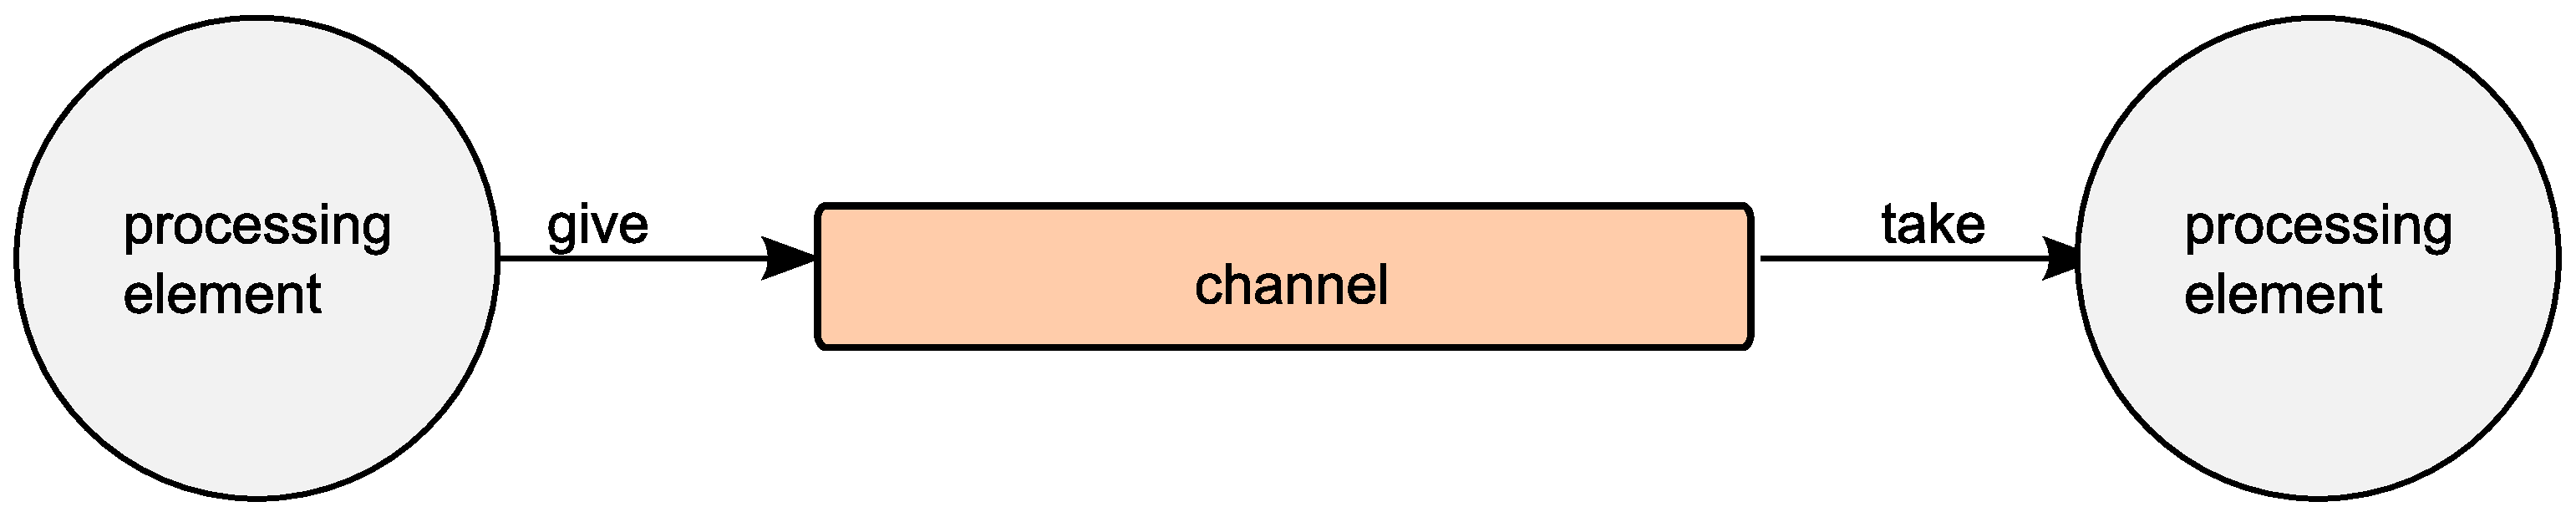
\includegraphics[width=\textwidth]{chapters/gcol/figs/cml_exchange.eps}
    \caption[Diagram of the message-passing primitive in \glsentrylong{cml-glossary}]{In \gls{cml}, logical processing elements synchronously exchange values over channels.  When one processing element offers to give a value on a channel, and another offers to take a value on the same channel, they ‘rendezvous’ and exchange the value as a passed message.}
    \label{fig:gcol:cml_exchange}
\end{figure}

% We were interested in exploring \gls{cml} as another methodology to use for simulating \gls{ps} where communication is involved.  For a first experiment, we chose to implement Gheorghe \textit{et al.}'s 3-colouring problem solution from \cite{Gheorghe2013}, as it involves communication between compartments but is relatively low-complexity and thus appears to be suitable for a first attempt.

% We chose to use the programming language \fsharp{} with the library Hopac,\footnote{\url{https://github.com/Hopac/Hopac}} which is modelled on \gls{cml} and follows it closely.\footnote{The final program can be found at \url{https://github.com/jcoo092/acmc2018}}  `Record' types are used to represent the individual compartments described in \cite{Gheorghe2013}.  The program then advances through multiple steps, applying the rules (encoded as functions that operate on the record types) in accordance with \cite{Gheorghe2013}.  Finally, once a solution is found, or found not to be possible, that is communicated to the environment.

% Insofar as possible, our implementation has been created to follow the algorithm described in \cite{Gheorghe2013} faithfully, and thus perhaps is not optimal in its efficiency, as an idiomatic specification of a Simple Kernel P~system does not necessarily match to the idiomatic or efficient form of an \fsharp{} program.  That is, we have written the program to prioritise staying as close to the original \gls{skps} model as possible, rather than writing the program to suit the strengths and typical style of the host language.  Consequently, the efficiency of the program may be worse than it could be otherwise. 

This \namecref{sec:gcol:cml} explores \gls{cml} as another methodology to use for simulating \gls{ps} where communication is involved.  For a first experiment, it implements \citeauthor{Gheorghe2013}'s 3-colouring problem solution from \cite{Gheorghe2013}, as it involves communication between compartments but is relatively low-complexity and thus appears to be suitable for a first attempt at simulating communicating \gls{ps} with \gls{cml}.

The programming language \fsharp{} was used with the library Hopac,\footnote{\url{https://github.com/Hopac/Hopac}} which is modelled on \gls{cml} and follows it closely.\footnote{The final program can be found at \url{https://github.com/jcoo092/acmc2018}}  `Record' types are used to represent the individual compartments described in \cite{Gheorghe2013}.  The program then advances through multiple steps, applying the rules (encoded as functions that operate on the record types) in accordance with \cite{Gheorghe2013}.  Finally, once a solution is found, or found not to be possible, that is communicated to the environment.

Insofar as possible, the implementation follows the algorithm described in \cite{Gheorghe2013} faithfully, and thus perhaps is not optimal in its efficiency, as an idiomatic specification of a Simple Kernel P~system does not necessarily match to the idiomatic or efficient form of an \fsharp{} program.  That is, the program prioritises staying as close to the original \gls{skps} model as possible, rather than adapting to suit the strengths and typical style of \fsharp{}.  Consequently, the efficiency of the program may be worse than it could be otherwise.

Ultimately, however, this example is relatively trivial and involves little communication, and therefore does not test the use of \gls{cml} significantly.  Much of the operation of the algorithm in fact does not involve communication between different compartments/processing elements at all.  Instead, it is primarily based in the evolution of objects contained within the compartments, with minimal communication between compartments at the end.  While that is highly effective in \gls{ps} \cite{Paun2008}, it would be interesting to see the results of using \gls{cml} for other problems where synchronous communication\footnote{While \gls{cml} uses synchronous communication by default, it is also relatively simple to implement asynchronous communication also using it if desired \cite{Reppy2007}.} is a much bigger part of the evolution of the system.

In common with most ad-hoc simulations, while the implementation is reasonably successful, it is not particularly customisable, and the code as written does not comport as precisely to the appearance of the theoretical rules of the \gls{skps}~system as the \gls{plingua} version created for \cite{Gheorghe2013} does.  Neither does the current implementation have any form of verification or invariant detection, as provided by \gls{mecosim} \cite{Perez-Hurtado2010} and Spin \cite{Ben-Ari2008,Lefticaru2011}.%  It would be worthwhile to pursue future work that seeks to improve one implementation/simulation by incorporating relevant parts of the other.

\gls{cml} seems to match to \gls{skps} well, but also looks like it might fit well with \gls{tlps} with symport/antiport \cite{Verlan2005} as well perhaps as \gls{tlps} with Channel States \cite{Song2016}, and Generalized Communicating \gls{ps} with minimal interaction rules \cite{Csuhaj-Varju2011}.  It would also appear to be a good fit for \gls{snps} \cite{Ionescu2006}, though \gls{cml} would probably be `overkill' for \gls{snps}.  In general, any variant of \gls{ps} which heavily uses synchronous communication between different cells/neurons/non-nested membranes/etc. over well-defined channels may be amenable to a \gls{cml} implementation.

Technically, the base form of \gls{cml} would only support antiport (i.e. one-way synchronous communication), but it is fairly simple to build two-way communication on top of it \cite[ch.~6]{Reppy2007}.  No attempt to model other systems has been made yet, however.

\subsection{Simulation results}
The program's running time on a number of differing graphs were recorded, with red, green and blue as the set of colours with which to colour the graphs.  The desktop computer used for these simulations has a four-core 3.6GHz Intel Core i7-7700 CPU, with 16 GB of RAM, running Windows 10, build number 10.0.17134.228.  The \fsharp{} programs were compiled and run on .NET Core 2.1.4, while \gls{mecosim} was run on Java version 8, build 1.8.0\_201-b09. 

% We recorded our program's running time on a number of differing graphs, with red, green and blue as our set of colours with which to colour the graphs.  The desktop computer used for these simulations has a four-core 3.6GHz Intel Core i7-7700 CPU, with \qty{16}{\giga\byte} of RAM, running Windows 10, build number 10.0.17134.228.  Our \fsharp{} programs were run on .NET Core 2.1.4, while \gls{mecosim} was run on Java version 8, build 1.8.0\_201-b09.

The first simulation used the graph shown in Figure 2 of \cite{Gheorghe2013}, reproduced here as \cref{fig:gcol:gheorghefig2}, which took 2.6s to process.  In keeping with that paper and following its definition of \(G(N,q)\), where \(G(N,q)\) is used to represent a graph of \(N\) nodes with all other nodes connected only to node \(q\) in a hub-and-spoke formation,\footnote{This is different to the random graphs that are also commonly denoted by this notation.} the graphs \(G(10,1)\) and \(G(10,10)\) (see \cref{fig:gcol:gs}) were also tested, finding that 0.3s is required for each.  The simulation was also tested using the classic \emph{Petersen graph}, shown in \cref{fig:gcol:petersen}, and found that it too required approximately 0.3s.

\begin{figure}
    \centering
    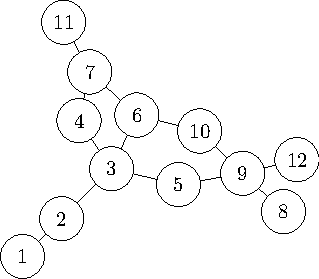
\includegraphics[width=0.65\textwidth]{chapters/gcol/figs/gheorghe-figure-2-figure0.pdf}
    \caption[A reproduction of the graph in Figure 2 of \cite{Gheorghe2013}]{\label{fig:gcol:gheorghefig2}A reproduction of Figure 2 from \cite{Gheorghe2013}.  Although this figure and Figure 2 in \cite{Gheorghe2013} are visually distinct, the graphs are isomorphic.}
\end{figure}

\begin{figure}
    \centering
    \begin{subfigure}[b]{0.35\textwidth}
        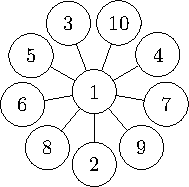
\includegraphics[width=\textwidth]{chapters/gcol/figs/g-10-1.pdf}
        \caption{\label{fig:gcol:g-10-1}\(G(10,1)\)}
    \end{subfigure}
    \hfill
    \begin{subfigure}[b]{0.35\textwidth}
        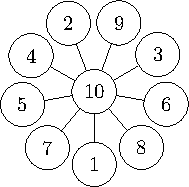
\includegraphics[width=\textwidth]{chapters/gcol/figs/g-10-10.pdf}
        \caption{\label{fig:gcol:g-10-10}\(G(10,10)\)}
    \end{subfigure}
    \caption[Graphs representing \(G(10,1)\) and \(G(10,10)\)]{\label{fig:gcol:gs}Graphs representing (a) \(G(10,1)\) and (b) \(G(10,10)\), as described in \cite{Gheorghe2013}, where the first number represents the size of the graph, and the second number represents the label of the centre node of the graph, with all other nodes connected only to that node.}
\end{figure}

\begin{figure}
    \centering
    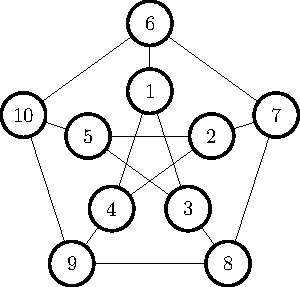
\includegraphics[width=0.45\textwidth]{chapters/gcol/figs/petersen-figure0.pdf}
    \caption[The Petersen Graph]{\label{fig:gcol:petersen}The classic Petersen graph, with nodes labelled 1 to 10.}
\end{figure}

Further simulations were run on complete graphs.  For a complete graph of \(N = 10\), the algorithm again required 0.3s.  It was then tried on a complete graph of \(N = 20\), but the test had to be aborted after a matter of minutes due to the computer running out of memory.  Running times of 0.83s, 2.6s, 8.88s, 26.6s and 84s for \(N = 11, 12, 13, 14\) and \(15\), respectively, were recorded.  Given that significant jumps in memory use were observed while running the larger graphs, it appears that the major cause of the rapid slowdown is likely to do with frequent ad-hoc memory allocations and de-allocations, though this was not profiled in detail.

% Gheorghe \textit{et al.} state \cite[p.~828]{Gheorghe2013} that in the latest version of \gls{plingua} at the time of writing, a strategy of eliminating compartments for which there can be no further rule applications is employed.  Using said strategy, results are typically achieved quite quickly.  It has the effect of pruning the search space, and reduces the total running time in some instances to just one-fifth of the running time of the simulation without such dead-compartment-elimination.

\citeauthor{Gheorghe2013} state \cite[p.~828]{Gheorghe2013} that in the latest version of \gls{plingua} at the time of writing, a strategy of eliminating compartments for which there can be no further rule applications is employed.  Using said strategy, results are typically achieved quite quickly.  It has the effect of pruning the search space, and reduces the total running time in some instances to just one-fifth of the running time of the simulation without such dead-compartment-elimination.

The \fsharp{} program does not choose which compartments to operate upon in the same fashion, but applying the colour guard on rule \(r_{2,2n+1}\) of the \gls{skps}~system throughout the process results in the pruning of compartments which already contain invalid results and thus can be eliminated safely. Therefore, to achieve the same effect as with \gls{plingua}'s strategy, this guard was used while applying rule \(r_{2,2n+1}\) and the result used to filter out all invalid compartments.  Doing this reduces the evaluation of complete graphs to around 60 milliseconds or slightly more, since every compartment in them can always be eliminated once colours have been assigned to four nodes.  It also reduces the running time of \cref{fig:gcol:gheorghefig2} to around 0.25s, and the Petersen graph, \(G(10,1)\) and \(G(10,10)\) to 0.1s.

\subsubsection{Comparison with original results}

\Cref{tab:gcol:timings} compares the timing results of the simulations reported in \cite{Gheorghe2013}, as well as the results of using \gls{mecosim}\footnote{The latest version of \gls{mecosim} available from \url{http://www.p-lingua.org/mecosim/} as at 10 January 2019 was used.} \cite{Perez-Hurtado2010} to re-run the same simulations locally on the same computer used to time the \fsharp{} solution, with the timing results mentioned above.

\begin{table}
\centering
\begin{tabular}{@{}lcccc@{}}
\toprule
Graph       & \begin{tabular}[c]{@{}c@{}}\gls{plingua}\\ (original)\end{tabular} & \begin{tabular}[c]{@{}c@{}}\gls{plingua}\\ (local)\end{tabular} & CML   & \begin{tabular}[c]{@{}c@{}}CML with\\ pruning\end{tabular} \\ \midrule
Fig. 2      & N/A                                                           & 17.0                                                           & 2.6  & 0.25                                                 \\
Petersen    & N/A                                                           & 1.5                                                       & 0.3  & 0.1                                                       \\
G(10,1)     & 7                                                            & 2.6                                                           & 0.3  & 0.1                                                       \\
G(10,10)    & \textgreater 4 min                             & N/A                                                           & 0.3  & 0.1                                                       \\
Complete 11 & 5                                                            & 0.15                                                           & 0.83 & .06                                                       \\
Complete 12 & 5                                                            & 0.15                                                           & 2.6  & .06                                                       \\
Complete 13 & 5                                                            & 0.15                                                           & 8.88 & .06                                                       \\
Complete 14 & 5                                                            & 0.15                                                           & 26.6 & .06                                                       \\
Complete 15 & 5                                                            & 0.15                                                           & 84   & .06                                                       \\ \bottomrule
\end{tabular}%
\caption[Comparison of recorded timings between \cite{Gheorghe2013} and this work]{Comparison of recorded timings between \cite{Gheorghe2013} and this work.  All measurements are in seconds, unless otherwise stated.  Where more than one result was reported in \cite{Gheorghe2013} for the same graph, the shortest running time has been included here.}
\label{tab:gcol:timings}
\end{table}

Attempts to run the simulation of \(G(10,10)\) in \gls{mecosim} repeatedly failed with an out-of-memory error.  Why this should be the case is uncertain, given that in the other instances, executions of the \gls{mecosim} \gls{skps} simulations achieved lower runtimes than those of \cite{Gheorghe2013}.  The execution of \(G(10,10)\) notwithstanding, the overall improvements in runtime of the \glspl{skps} are likely due to a combination of the computer used locally being more recent and thus likely more powerful, and improvements in the underlying \gls{mecosim} and \gls{plingua} software.

It seems odd, however, that two functionally identical graphs, \(G(10,1)\) and \(G(10,10)\), would have such dramatically different run time behaviours when running in \gls{mecosim} --- seen in both the original and reproduced local results.  This might be due to an unusual performance bug hidden deep within \gls{mecosim}, though this was not investigated further.

These results appear to suggest that the \fsharp{} implementation generally provides superior running time results, though it was not tested on a particularly wide variety of scenarios.  Extrapolating from the collected results, it seems plausible that the scenarios that would result in the longest running time will likely be those that have a moderate level of connectedness in the graph.  Highly connected graphs will likely see many potential paths eliminated early due to frequent occurrences of colour conflicts, while graphs with few connections will have relatively few potential paths to explore.

The \fsharp{} results and those of the \gls{mecosim} simulations are not \emph{completely} comparable, however.  The \fsharp{} solution was programmed directly to follow the \gls{skps} system's rules, whereas the \gls{mecosim} solution was specified as the \gls{skps}~system rules in \gls{plingua}, with the operation of the computer simulation carried out by \gls{mecosim}.  This difference between `ad-hoc' and `general' simulation means that one would expect to see the \fsharp{} simulation achieve better results from the outset, as overheads that accompany a general simulation implementation can be avoided.\footnote{One could see ad-hoc as being akin to running a program compiled to native instructions, while using a general simulation is similar, in principle, to running a program in an interpreter.  The latter is typically simpler to work with and more portable, but comes with overheads that slow down execution.}  \Gls{mecosim} is an excellent tool, and, combined with \gls{plingua}, it provides a valuable service to the Membrane Computing community in that it allows researchers to validate their systems and rulesets while staying close to their mathematical descriptions, and without having to delve into the details of implementing a given algorithm in code.  See further \cite{Perez-Hurtado2019} for more of a discussion on ad-hoc and general simulations, and a narrowing of the differences between the two.